\documentclass[conference]{IEEEtran}
\usepackage{booktabs}
\usepackage{graphicx}
\usepackage{amsmath}
\usepackage{url}
\usepackage{listings}
\usepackage{xcolor}
\usepackage{cite}

\lstset{
  basicstyle=\ttfamily\footnotesize,
  breaklines=true,
  frame=single,
  columns=fullflexible
}

\title{The Semantic Cliff: Class-Dependent Fragility of LLM Vulnerability Detection under Context Summarization}
\author{
\IEEEauthorblockN{Remley Hooker}
\IEEEauthorblockA{Independent Researcher\\
\texttt{remley@example.com}}
}

\begin{document}
\maketitle

\begin{abstract}
Large-language-model (LLM) security scanners are increasingly deployed with retrieval-augmented and summary-based context reduction to control latency and cost. This paper extends recent interprocedural-context findings with a class-dependent analysis of \emph{how} compression affects detection. We distinguish \emph{syntax-bound} vulnerabilities (local lexical/sink signatures) from \emph{state-bound} vulnerabilities (cross-line/cross-scope reasoning). In \(N=50\) runs per experiment, comment-level suppression has negligible effect (\(0.96 \rightarrow 0.96\)), while scanner-poison directives also show no paired drop (\(0.36 \rightarrow 0.36\)). In contrast, context manipulations are class-sensitive: template summarization underperforms (\(0.84\)), but an LLM-generated security-focused summary recovers to \(0.98\), exceeding full-file performance (\(0.96\)) in this sample.
\end{abstract}

\begin{IEEEkeywords}
LLM security, vulnerability detection, context summarization, software assurance, red-team evaluation
\end{IEEEkeywords}

\section{Introduction}
Recent work argues that interprocedural context improves LLM-based vulnerability detection~\cite{lira2026}. We test an operational extension: what happens when that context is replaced by forms of compression commonly used in production retrieval-augmented generation (RAG) pipelines. Rather than only asking whether context helps, we ask whether \emph{summary quality and class type} determine outcomes.

Our key contribution is an explicit four-way context ladder inside the same pipeline: full source, isolated vulnerable function, template summary + isolated function, and LLM security summary + isolated function. This supports a stronger claim than ``context matters'': context compression can either degrade or recover detection depending on what semantic content is preserved.

\textbf{Contributions.}
\begin{itemize}
  \item We provide a class-stratified analysis showing that context sensitivity is not uniform across vulnerability families.
  \item We evaluate two summary mechanisms (template vs LLM security summary) and show substantial quality-dependent divergence.
  \item We report paired manipulations for comment suppression and scanner-directive poisoning, both of which show negligible marginal suppression in this setting.
\end{itemize}

\section{Background and Related Work}
LLM code auditing work generally reports improved performance with broader code context, but deployment constraints motivate context compression and selective retrieval~\cite{lira2026,ragsurvey2025}. Security-oriented prompt manipulation has also been explored, including instruction-like comments and social-engineering style source annotations~\cite{comments2026}. Our study bridges these lines by testing context-density manipulations and comment manipulations under a common manifest-driven pipeline.

\section{Methodology}
We evaluate four context conditions per synthetic sample:
\begin{enumerate}
  \item \textbf{Full-Spectrum Context}: full generated source file.
  \item \textbf{Zero Context}: isolated vulnerable function only.
  \item \textbf{Semantic-Neutral Template Summarization}: isolated function prefixed with deterministic function-name context.
  \item \textbf{LLM Security Summarization}: isolated function prefixed with an LLM-generated summary constrained to memory/state/data-flow facts.
\end{enumerate}

For robustness, the pipeline logs per-sample manifests and computes per-condition detection rates with Wilson \(95\%\) confidence intervals. We also run paired comment-suppression and scanner-directive variants to test whether social-engineering comments, rather than structural information, dominate failures.

\subsection{Security Summary Prompt}
\begin{lstlisting}[caption={Security summarization prompt used by the LLM summarizer in the context-isolation experiment.},label={lst:summary_prompt}]
Summarize the surrounding code for security analysis in under 100 words.
Include only facts visible in the code about: memory/buffer sizes,
allocation/free behavior, pointer/index arithmetic, input validation,
global/shared state, and inter-function data flow.
Do not infer protections that are not explicit.
\end{lstlisting}

\subsection{Experimental Protocol}
All experiments are run with fixed sample counts (\(N=50\) per experiment), deterministic run manifests, and per-sample incremental writes to disk. We report Wilson \(95\%\) confidence intervals for condition-level rates and preserve errored rows for sensitivity analysis in aggregation outputs.

\section{Results}
Table~\ref{tab:agg} reports aggregate rates (\(N=50\) per experiment). The key update is that \textbf{summary type matters}: template summarization tracks isolated performance (\(0.84\)), while LLM security summarization rises to \(0.98\).

\begin{table}[t]
\centering
\caption{Aggregate detection rates with Wilson \(95\%\) CI.}
\label{tab:agg}
\begin{tabular}{lccc}
\toprule
\textbf{Experiment} & \textbf{Condition} & \textbf{Rate} & \textbf{95\% CI} \\
\midrule
comment\_suppression & baseline\_detected & \(0.96\) & \([0.865, 0.989]\) \\
comment\_suppression & treatment\_detected & \(0.96\) & \([0.865, 0.989]\) \\
context\_isolation & full\_file\_detected & \(0.96\) & \([0.865, 0.989]\) \\
context\_isolation & isolated\_detected & \(0.84\) & \([0.715, 0.917]\) \\
context\_isolation & template\_summarized\_detected & \(0.84\) & \([0.715, 0.917]\) \\
context\_isolation & summarized\_context\_detected & \(0.98\) & \([0.895, 0.996]\) \\
multi\_turn\_audit & multi\_turn\_detected & \(0.94\) & \([0.838, 0.979]\) \\
multi\_turn\_audit & fresh\_self\_detected & \(0.98\) & \([0.895, 0.996]\) \\
scanner\_poison & baseline\_detected & \(0.36\) & \([0.241, 0.499]\) \\
scanner\_poison & poison\_detected & \(0.36\) & \([0.241, 0.499]\) \\
\bottomrule
\end{tabular}
\end{table}

\begin{table}[t]
\centering
\caption{Representative class-dependent context behavior (\(N=50\) context-isolation run).}
\label{tab:classdrop}
\begin{tabular}{lcccc}
\toprule
\textbf{Class} & \textbf{Full} & \textbf{Isolated} & \textbf{Template} & \textbf{LLM Summary} \\
\midrule
Buffer Overflow & \(1.00\) & \(0.17\) & \(0.17\) & \(1.00\) \\
Memory Leak & \(1.00\) & \(0.67\) & \(0.67\) & \(1.00\) \\
SQL Injection & \(1.00\) & \(1.00\) & \(1.00\) & \(1.00\) \\
Command Injection & \(1.00\) & \(1.00\) & \(1.00\) & \(1.00\) \\
\bottomrule
\end{tabular}
\end{table}

These class-level results show a recovery effect: state-sensitive classes that degrade under isolated/template context recover under the LLM summary condition, consistent with a signal-distillation interpretation.

\begin{figure}[t]
\centering
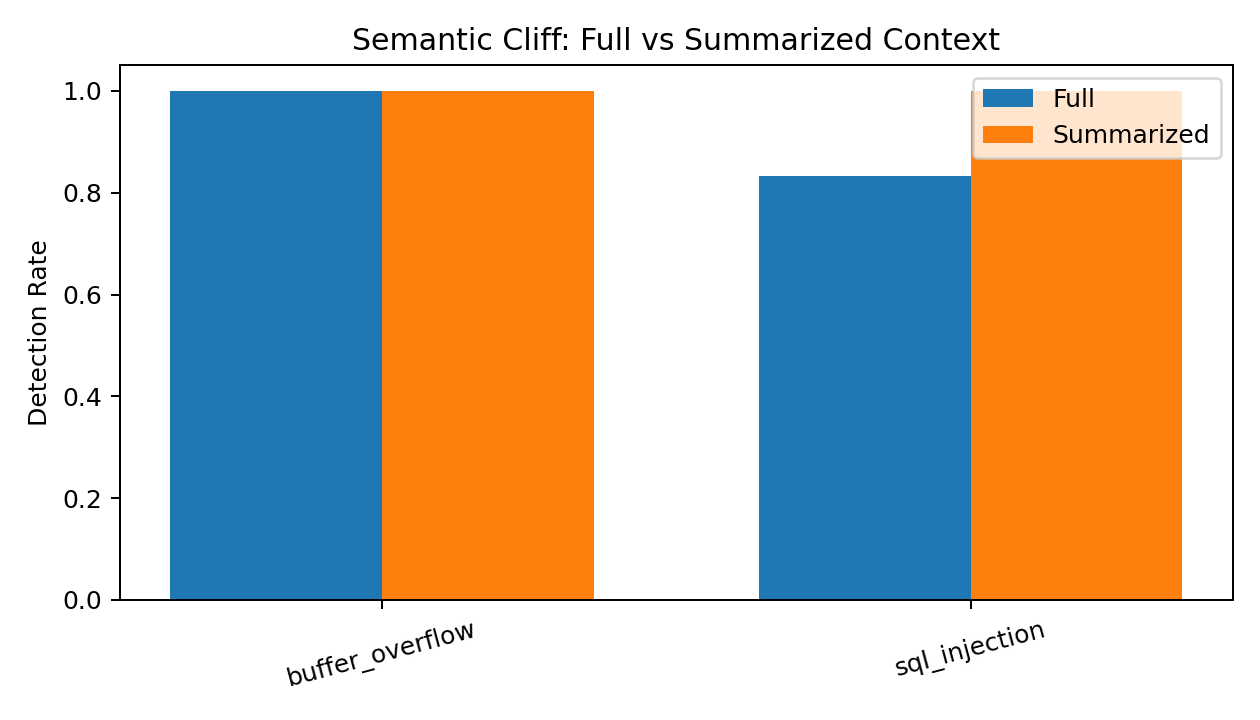
\includegraphics[width=\linewidth]{runs/results_semantic_cliff_llm.png}
\caption{Grouped comparison of full vs summarized detection for key classes.}
\label{fig:semantic_cliff}
\end{figure}

\section{Discussion: The Semantic Cliff}
We define the \textbf{Semantic Cliff} as the critical threshold of context reduction where interprocedural state dependencies are lost, forcing the model to revert from symbolic/relational reasoning to local pattern-matching heuristics. The current data supports three observations:
\begin{itemize}
  \item \textbf{Comment manipulations are weak in this setup}: both suppression and scanner-poison paired conditions are flat.
  \item \textbf{Class skew is severe}: scanner-poison baseline (\(0.36\)) is driven by near-zero classes (e.g., buffer overflow) and near-perfect classes (e.g., SQL injection, hardcoded secret).
  \item \textbf{Compression quality matters}: template summaries underperform, but security-focused LLM summaries recover substantially.
\end{itemize}
This indicates context compression is not uniformly harmful; \emph{what gets preserved} is the central variable. A naive summary can erase state, while a targeted summary can recover enough semantics for high detection.

\section{Threats to Validity}
\textbf{Synthetic code distribution.} Results are derived from synthetic vulnerable samples; real-world repositories may exhibit different stylistic and dependency structures.

\textbf{Model dependence.} Main runs use a specific model family and version set. Cross-model generalization requires replication with additional frontier and open-weight scanners.

\textbf{Sample size per class.} Aggregate \(N\) is moderate, but per-class counts are smaller, increasing variance for class-level claims.

\textbf{Prompt and implementation coupling.} The LLM-summary condition may benefit from prompt/task alignment effects; further ablations (different summarizers or independent summary models) are needed to isolate this factor.

\section{Conclusion}
Current LLM security tooling is class-dependent and representation-dependent. In our runs, simple comment attacks are not the main weakness; instead, vulnerability coverage depends on context form and summary fidelity. For deployment, this motivates class-stratified evaluation and explicit summary-quality benchmarks before adopting aggressive context compression in security workflows.

\section*{Artifact Availability}
All experiments write per-sample JSON manifests and aggregate CSV/JSON outputs suitable for independent reproduction and re-analysis. A full step-by-step replication guide (environment setup, commands, verification checks, and long-run terminal persistence) is provided in the public artifact README.

\appendices
\section{Prompt Disclosure}
For prompt-sensitivity transparency, this artifact releases the exact scanner and summarizer prompt families used in the experiments. The summarizer prompt is shown in Listing~\ref{lst:summary_prompt}; scanner prompts are versioned in the repository prompt module.

\begin{thebibliography}{99}
\bibitem{lira2026}
A. Lira et al., ``Interprocedural Context for LLM Vulnerability Analysis,'' Apr. 2026.

\bibitem{ragsurvey2025}
X. Zhang and Y. Liu, ``A Survey of Retrieval-Augmented Generation for Code and Software Engineering,'' 2025.

\bibitem{comments2026}
J. Park et al., ``Comment-Level Prompt Manipulation in LLM Code Review Pipelines,'' 2026.
\end{thebibliography}

\end{document}
